\documentclass[oribibl]{llncs}

% Other packages needed
\usepackage{newfloat}
\usepackage{cite}
\usepackage{chngcntr}
\counterwithout*{figure}{chapter} % make sure figures are numbered right
\DeclareFloatingEnvironment[  % create the Model float
  fileext=los,
  listname=List of Models,
  name=Model,
  placement=tbhp,
  within=section
]{model}
\usepackage{amsmath, amssymb, amsfonts}  % include math packages
\let\doendproof\endproof
\renewcommand\endproof{~\hfill\qed\doendproof} % put square at end of proofs

\usepackage{graphicx,booktabs,multirow,tabu} % include general stuff

% shortcuts etc.
\def\Lmax{{L_{\mathrm{max}}}}

\begin{document}
% Title
\title{A New MIP Model for Parallel-Batch Scheduling with Non-Identical Job Sizes}
\author{Sebastian Kosch \and J. Christopher Beck}
\institute{University of Toronto\\Dept. of Mechanical and Industrial
Engineering\\\email{\{skosch,jcb\}@mie.utoronto.ca}}

\maketitle

\begin{abstract}
  Parallel batch machine problems arise in numerous manufacturing
  settings. They have recently been addressed by Malapert et al., who
  proposed the implementation of a new \texttt{sequenceEDD} global
  constraint. The latter, in combination with \texttt{pack}, forms the
  current state-of-the-art approach and performs significantly better
  than a basic MIP formulation of the problem. In this paper, we present
  three improvements to this basic MIP model and show that they boost its
  performance and solution quality to match and exceed that of the CP
  model.

  \textbf{$\uparrow\quad$ CB: To be fixed later.}
\end{abstract}

\section{Introduction}

Despite the widespread application of mixed integer programming (MIP)
technology to optimization problems in general and scheduling problems
specifically,\footnote{For example, of the 58 papers published in the
\emph{Journal of Scheduling} in 2012, 19 use MIP, more than any other
single approach.} there is a significant body of work that demonstrates
the superiority of constraint programming (CP) and hybrid approaches for
a number of classes of scheduling problems \cite{some_sched_papers}.
While the superiority is often a result of strong inference techniques
embedded in global constraints \cite{cumulative}, the strong performance
is often the result of more detailed, problem-specific implementation in
the form of specialized global constraints \cite{Malapert} or
instantiations of decomposition techniques \cite{Hooker_etc}. The
flexibility of CP and hybrid techniques which facilitates such
implementation is undoubtedly positive from the perspective of solving
specific problems better. However, the flexibility is in some ways in
opposition to the ``holy grail'' of CP \cite{Freuder97a}: to enable
users to model and solve problems without implementing anything new at
all.

Our over-arching thesis is that, in fact, MIP technology is closer to
this goal than CP, at least in the context of combinatorial optimization
problems. In our investigation of this thesis, we are developing MIP
models for scheduling problems where the current state of the art is
customized CP or hybrid approaches. Heinz et al. \cite{Heinz} showed
that on a class of resource allocation and scheduling problems, a MIP
model could be designed that was competitive with the state-of-the-art
logic-based Benders decomposition approach. This paper represents a
similar contribution in different scheduling problem: a parallel batch
processing problem which has previously been attacked by MIP,
branch-and-price \cite{Daste1}, and CP \cite{Malapert}. The latter represents
the current state of the art.

In this paper, we propose a MIP model inspired by the idea of modifying
a canonical sub-optimal solution to arrive at an optimal solution.
The definition of our objective function in this novel context is not
intuitive until we reason algorithmically about how constraints and
assignments interact -- a strategy usually reserved for local search
techniques. Indeed, we suggest that the analogy between branching
on independent binary decision variables and making moves between
neighbouring schedules should be explored in more detail for a range of
combinatorial problems.

The balance of the paper is organized as follows. In next section we
present the formal problem definition and discuss existing approaches.
In Section \ref{sec:propositions} we present and
prove a number of propositions that allows us to propose a novel MIP
model for the problem before formally defining the model in Section
\ref{sec:newMIPmodel}. Section \ref{sec:exp} presents our empirical
results, demonstrating that the performance of the new model is superior
to the existing CP model, both in terms of mean time to find optimal solutions
and in terms of solution quality when optimal solutions could not be found
within the time limit.

\section{Background}
\label{sec:background}

Batch machines with limited capacity exist in many manufacturing
settings: as ovens in semiconductor manufacturing \cite{Lee}, autoclaves
in the production of carbon fiber parts \cite{Malapert}, and processing
tanks in the pharmaceutical industry \cite{Grossmann}. In this paper,
we tackle the problem of minimizing the maximum lateness, $\Lmax$,
in a single machine parallel batching problem where each job has an
individual due date and size.

We use the following notation: a set $\mathcal{J}$ of $n$ jobs,
is to be assigned to a set of batches $\mathcal{B} = \{B_1,\dots,B_n\}$. Every
job $j$ has three properties: its processing time $p_j$, its size $s_j$
and its due date $d_j$. Jobs can be assigned to arbitrary batches, as
long as the sum of the sizes of the jobs in any batch does not exceed
the machine capacity, $b$.

The single machine processes one batch at a time. Each batch $B_k$ has a
\textit{batch start date} $S_k$, a \textit{batch processing time},
defined as the longest of processing times of all jobs assigned to the
batch, $P_k = \max_{j\in \mathcal{B}_k}(p_j)$, and a \textit{batch completion
  date}, which must fall before the start time of the next batch, $C_k
= S_k + P_k \leq S_{k+1}$.

The lateness of a job $j$, $L_j$, is the completion time of its batch
$C_k$ less its due date $d_j$. The objective function is to minimize the
maximum lateness over all jobs, $\Lmax = \max_{j \in \mathcal{J}}(L_j)$. Since we
are interested in the maximum lateness, only the earliest-due job in
each batch matters and is referred to as the \textit{batch due date}
$D_k = \min_{j\in \mathcal{B}_k}(d_j)$.

Previous authors have used the format established by Graham et al.
\cite{graham} to summarize the problem as $1|\textit{p-batch}; b
< n; \textit{non-identical}|\Lmax$ \cite{Daste, Malapert}, where
$\textit{p-batch};b<n$ represents the parallel-batch nature and the
finite capacity of the resource. A simpler version with identical job
sizes was shown to be strongly NP-hard by Brucker et al. \cite{Brucker};
this problem, therefore, is no less difficult.

Figure \ref{fig:intro_tetris} shows a solution to a sample
problem with eight jobs and a resource with capacity $b = 20$. The last batch
has the maximum lateness $L_5 = C_5 - D_5 = 70 - 39 = 31$.

\begin{figure}[th]
\centering
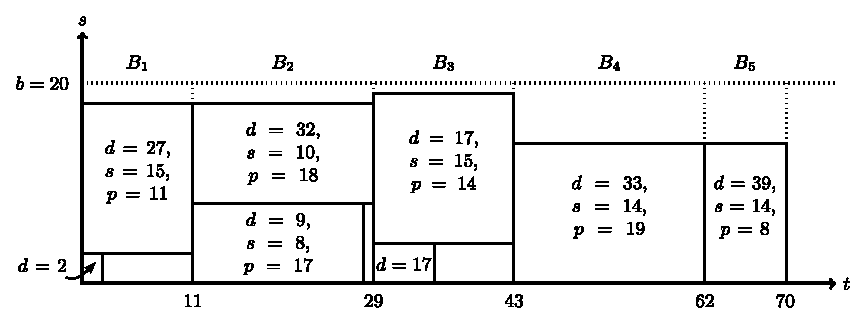
\includegraphics[width=\textwidth]{tetris.pdf}
\caption{An optimal solution to an example problem with eight jobs (values for
  $s_j$ and $p_j$ are not shown for the two small jobs in batches 1 and 3,
respectively).}
  \label{fig:intro_tetris}
\end{figure}

\subsection{Reference MIP model} The problem is formally defined by MIP
Model \ref{model:malapertmip}, used by Malapert et al. \cite{Malapert} for comparison
with their proposed CP model (see below).

\begin{model}[h]
\begin{alignat}{2}
\mathrm{Min.}\quad & \Lmax && \\
\mathrm{s.t.}\quad &\sum_{k \in \mathcal{B}} x_{jk} = 1 \quad && \forall j \in \mathcal{J}
\label{c:malapp-unique}\\
  &\sum_{j \in \mathcal{J}} s_j x_{jk} \leq b \quad && \forall k \in \mathcal{B}\label{c:malapp-cap}\\
  &p_j x_{jk} \leq P_k \quad && \forall j \in \mathcal{J}, \forall k \in
  K\label{c:malapp-pk}\\
  &C_{k-1} + P_{k} = C_k \quad && \forall k \in \mathcal{B}\label{c:malapp-ck}\\
  &(d_\mathrm{max} - d_j)(1 - x_{jk}) + d_j \geq D_k \quad && \forall j \in \mathcal{J}, \forall
  k \in \mathcal{B}\label{c:malapp-dk}\\
&C_k - D_k \leq \Lmax \quad && \forall k \in \mathcal{B}\label{c:malapp-lmax}\\
  &D_{k-1} \leq D_k \quad && \forall k \in \mathcal{B} \label{c:malapp-edd} \\%[2ex]
  &x_{jk} \in \{0,1\}, C_k \geq 0, P_k \geq 0, D_k \geq 0 \quad && \forall j \in \mathcal{J}, \forall k \in \mathcal{B}  
\end{alignat}
\caption{Reference MIP model}
\label{model:malapertmip}
\end{model}

The decision variable, $x_{jk}$ is a binary variable that is one
if and only if job $j$ is assigned to batch $k$. Constraints
\eqref{c:malapp-unique} ensure that each job $j$ is assigned to exactly
one batch $k$. Constraints \eqref{c:malapp-cap} ensure that no batch
exceeds the machine capacity, $b$. Constraints \eqref{c:malapp-pk}
define each batch's processing time $P_k$ as the maximum processing time
of the jobs $j$ assigned to it. Constraints \eqref{c:malapp-ck} define
each batch's completion time $C_k$ as that of the previous batch, plus
the batch's processing time. Constraints \eqref{c:malapp-lmax} define
the objective value $\Lmax$. Constraints \eqref{c:malapp-edd} sort the
batches by due date, based on a well-known dominance rule: there exists
an optimal solution with batches scheduled in earliest-due-date-first
order (EDD). This is due to the fact that if all jobs are already optimally
assigned, the problem reduces to a polynomial-time solvable single machine
problem ($1|D_k|\Lmax$) \cite{Pinedo03}.

\subsection{Previous Work}

Malapert et al. \cite{Malapert} present a CP formulation of the problem
(see Model \ref{model:malapertcp}) which relies on two
global constraints: \texttt{pack} \cite{Shaw04a}, which constrains the
job-to-batch assignments such that no capacity limits are violated,
and \texttt{sequenceEDD}, which enforces the EDD order over the batches. The
implementation of the latter constraint is the main contribution of
the paper and is primarily responsible for the strong performance. It
includes a set of rules which update the lower and upper bounds on
$\Lmax$ and on the number of batches every time \texttt{sequenceEDD}
is triggered by a job-batch assignment. Based on these bounds, other
assignments are then eliminated from the set of feasible assignments.

\begin{model}
  \label{model:malapertcp}
  \begin{alignat}{2}
    \mathrm{Min.}\quad & \Lmax &&  \\
    \mathrm{s.t.}\quad \label{c:mcpmax} & \mathtt{maxOfASet}(P_k, B_k, [p_j]_k,
    0) && \quad \forall k \in \mathcal{B} \\
    \label{c:mcpmin} & \mathtt{minOfASet}(D_k, B_k, [d_j]_k, d_\mathrm{max}) &&
    \quad \forall k \in \mathcal{B} \\
    \label{c:mcppack} & \mathtt{pack}(B_k, A_j, S_k, M, s_j) && \\
    \label{c:mcpseq} & \mathtt{sequenceEDD}(B_k, D_k, P_k, M, \Lmax)
    && \\
\end{alignat}
  \caption{CP model proposed by Malapert et al.}
\end{model}

Constraints \eqref{c:mcpmax} define $P_k$ as the maximum of the set
of processing times $[p_j]_k$ belonging to the jobs assigned to
batch $B_k$, with a minimum value of 0 (note that the notation is
adapted from Malapert et al. to match that in this paper). Constraints
\eqref{c:mcpmin} define $D_k$ as the minimium of the due dates $[d_j]_k$
associated with the set of jobs assigned to the batch $B_k$, with a
maximum of $d_\mathrm{max}$, the largest due date among all given jobs.
Constraint \eqref{eqc:mcppack} implements the limited batch capacity $b$.
It uses propagation rules incorporating knapsack-based reasoning, as
well as a dynamic lower bound on the number of non-empty batches $M$
\cite{Malapert,ShawPacking}. Note that this constraint handles the
channeling between the set of jobs assigned to batch $B_k$, and the
assigned batch index $A_j$ for each job $j$. The limited capacity is
enforced by setting the domain of the batch loads $S_k$ to $[0, b]$.
Constraint \eqref{c:mcpseq} ensures that the objective value $\Lmax$ is
equal to the maximum lateness of the batches scheduled according to the
EDD rule.

The problem has also been addressed with a detailed branch-and-price
algorithm \cite{Daste1}, which is described in \cite{Malapert} as
follows: each batch is a column in the column generation master
problem. A solution of the master problem is a feasible sequence of
batches. The objective of the subproblem is to find a batch which
improves the current solution of the master problem. Malapert et al.
\cite{Malapert} showed that their CP model, was significantly faster
than the branch-and-price algorithm which itself was more efficient 
than the reference MIP model. 

\textbf{$\uparrow\quad$ CB: I emailed Christelle Guéret about the B\&P paper,
but haven't heard back from her yet. I'll keep you posted.}

Other authors have examined similar problems: Azizoglu \& Webster
\cite{Azizoglu} provide an exact method and a heuristic for the same
problem, but minimize makespan ($C_\mathrm{max}$) instead of $\Lmax$,
similarly to the work by Dupont and Dhaenens-Flipo \cite{Dupont}.
Exact methods have been proposed for multi-agent variants
with different objective functions by Sabouni and Jolai \cite{Sabouni},
for makespan minimization on single batch machines by Kashan et al.
\cite{Kashan}, and for makespan minimization on parallel batch machines
with different release dates \cite{Ozturk}. A more
extensive review of MIP models in batch processing is given
by Grossmann \cite{Grossmann}. 

\section{Exploiting the Structure of the Parallel-Batching Problem}
\label{sec:propositions}

In this section, we provide a series of observations about the
parallel-batch scheduling problem that allow us to improve the reference MIP
model significantly.

\subsection{The single-EDD schedule and assigning jobs to earlier batches}
We can exploit the EDD rule to eliminate $\frac{1}{2}(n^2 - n)$ of the
$n^2$ potential job-batch assignments a priori.

We first re-index all jobs in non-decreasing due date (and in
non-decreasing processing time in case of a tie), which can be done in
$\mathcal{O}(n \log n)$ time. For the remainder of this paper, consider
all jobs to be indexed in this way. We then introduce the notion of
the \textit{single-EDD} schedule, in which each batch $B_k$ contains the
\textit{single} job $j$ matching its index (i.e., $x_{jk}=1$ exactly when
$j=k$), such that EDD is always satisfied. We refer to $j$ as the \textit{host
job} of batch $B_k$, while other jobs assigned to $B_k$ are \textit{guest jobs}.

\begin{proposition} \label{prop:movebackonly}
There always exists an optimal solution among the schedules in which job $j$ is assigned to batch
$B_k \; \forall \,j \leq k$, i.e. among the schedules where jobs are either assigned to
their single-EDD batches or to earlier-due batches.
\end{proposition}
\begin{proof}
  We will show the inverse: all solutions in which jobs are assigned to batches
  scheduled after their single-EDD batches \textit{either} violate EDD
  \textit{or} have equivalent solutions (in terms of $\Lmax$)
  in which jobs are assigned to earlier batches only.

  Consider a schedule in which $B_k$ is the earliest-scheduled batch such that
  its host job $j$ is assigned to a later-scheduled batch $B_{k+m}$, which makes
  $D_{k+m} = d_j$.

  The schedule violates EDD if one or more batches $B_q$ are due after
  job $j$ (i.e. $D_q>d_j$) with $k\leq q<k+m$. This will always be the
  case when $B_k$ holds other jobs due later than $j$. Note that by the
  definition of $B_k$ as the earliest batch such that its host job is
  assigned to a later batch, none of the jobs assigned to it can be due
  before $d_j$.

  If the schedule does not violate EDD, we need to consider the following cases:
  \begin{itemize}
    \item{$B_k$ is empty, so $P_k = 0$. Since EDD is not violated, we
    know that $D_q = d_j\;\forall\;B_q, k \leq q \leq k+m$. In this case,
    we can instead assign all jobs from $B_{k+m}$ into $B_k$, such that
    $P_{k+m} = 0$. $\Lmax$ will stay constant, as the completion time of
    the last-scheduled of all batches due at $d_j$ does not change.}
    \item{$B_k$ is non-empty and due before $d_j$: inapplicable per definition
        of $B_k$ above.}
    \item{$B_k$ is non-empty and due at $D_k = d_j$ (although $j \notin B_k$), due
        to at least one job $g$ from a later-scheduled batch for which
        $d_g = d_j$, which is assigned to $B_k$. In this case, since $D_k
        = d_j = D_{k+m}$ and since EDD is not violated, \textit{all} batches $B_q$
        where $k \leq q \leq k+m$ must be due at $d_j$. But then we can re-order
        these batches such that their respective earliest-due jobs are once
        again assigned to their single-EDD indices. The jobs in $B_{k+m}$
        (including $j$) will be assigned to $B_k$ as a result. $\Lmax$
    is not affected by this re-assignment, as the completion time of the
    last-scheduled batch due
  at $d_j$ does not change.}
    \item{$B_k$ is non-empty and due after $d_j$: inapplicable as it violates
      EDD.}
  \end{itemize}
\end{proof}

We thus introduce the following constraint to exclude solutions
in which jobs are assigned to later batches than their single-EDD
batches.
\begin{alignat}{2}
  & x_{jk} = 0 \quad && \forall \{j \in \mathcal{J}, k \in \mathcal{B} | j < k\} \label{eq:mipnopp}
\end{alignat}

We can also show that in every non-empty batch $B_k$,
the earliest-due job $j$ must be the single-EDD job (such that $j =
k$). This means that when batch $B_k$'s host job $j$ is assigned to an
earlier batch, no other jobs can be assigned to $B_k$; a batch
that is \textit{host-less} must be empty. This requirement rests on the
following proposition:

\begin{proposition}\label{prop:nohostless}
There exists an optimal solution that has no host-less, non-empty batches.
\end{proposition}
\begin{proof}
Consider an optimal schedule, ordered by EDD, in which batch $B_k$ is the
last-scheduled batch which is host-less but non-empty: instead of its host job
$j$ (with $j=k$), only a set $G$ of later-due guest jobs is assigned
to $B_k$ (where $j \notin G$). Note that the earliest-due job $g$ in $G$ must have the same
due date as batch $B_{k+1}$: if it is due later, EDD is violated; if it
is due earlier, $G$ is not a set of later-due guest jobs. 

Since $B_k$ is the last host-less non-empty batch, job $g$'s own single-EDD
batch $B_g$ is empty ($P_g = 0$). Then we can re-assign the guest jobs
$G$ from $B_k$ into $B_g$, such that $g$ is again host job in its own
single-EDD batch. This re-assignment has no impact on $\Lmax$ since it
makes $P_k = 0$, resulting in the same completion time of the set of all
batches with batch due date $D = D_{k+1}$.
\end{proof}

The above proposition translates to the following constraint:
\begin{alignat}{2}
  && x_{kk} \geq x_{jk} \quad & \forall\{j \in \mathcal{J}, k \in \mathcal{B} |
j> k\}
\end{alignat}

\subsection{Using changes to the single-EDD schedule to calculate the objective value}
\label{sec:moves}

We can formulate each batch's lateness, $L_k$, as its pre-computed
lateness in the single-EDD schedule, modified by the assignment of jobs into and
out of batches $B_h, h \leq k$.

\textbf{$\uparrow\quad $CB: I understand that you want to get away
from talking about the reference model. My understanding is that my model is faster
mainly because it has fewer rows and columns. Is that a valid motivation to bring up
here (in whichever form) or too handwavy? (I'm not sure about cuts, for
example)}

We first define $\mathcal{B}^\star \subseteq \mathcal{B}$ as the set of batches
$B_k$ which, given any EDD schedule, are the last-scheduled among all batches
with due date $D_k$, since we can make the following observation:
\begin{proposition}
Given a set of batches with equal due date in a schedule, we only need
consider the lateness value of the one scheduled last.
\end{proposition}
\begin{proof}
  In an EDD ordering, the lateness value of the batch scheduled last is greater
  than (or equal to, in the case of an empty batch) the lateness values
  of all other batches sharing its due date as it has the latest completion
  date.
\end{proof}
This fact allows us to reduce the number of constraints defining $\Lmax$, as
we only need to consider batches $\mathcal{B}^\star$ as potential candidates for
$\Lmax$.

To simplify the following arguments, we also define the term
\textit{move} as the re-assignment of a job $j$ from its single-EDD
batch $B_k$ to an earlier batch $B_h, h < k$, such that $x_{jk}=0$ and $x_{jh}=1$ and $j$
is a guest job in $B_h$.
Any schedule can thus be understood as a set $M$ of such moves, executed in arbitrary
order starting from the single-EDD schedule. To define the objective function,
we consider below the change in $\Lmax$ associated with individiual moves, going
from one schedule to another, instead of reasoning about the $\Lmax$ value of an entire schedule at once.

Consider any EDD
schedule, such as the one shown in Figure \ref{fig:movebasedmip}a. Moving
a job $j$ from its single-EDD batch $B_{k=j}$ into an earlier batch
$B_e$ has the following effect:

\begin{itemize}
\item{the lateness of all batches $B_i, i \geq k$ is reduced by $p_j$,
    as in Figure \ref{fig:movebasedmip}(b),}
\item{the lateness of all batches $B_h, h \geq e$ is increased by
$\max(0,p_j - P_e)$, where $P_e$ is the processing time of batch $B_e$
before $j$ is moved into it, as in Figure \ref{fig:movebasedmip}(c).}
\end{itemize}

\begin{figure}[th]
\centering
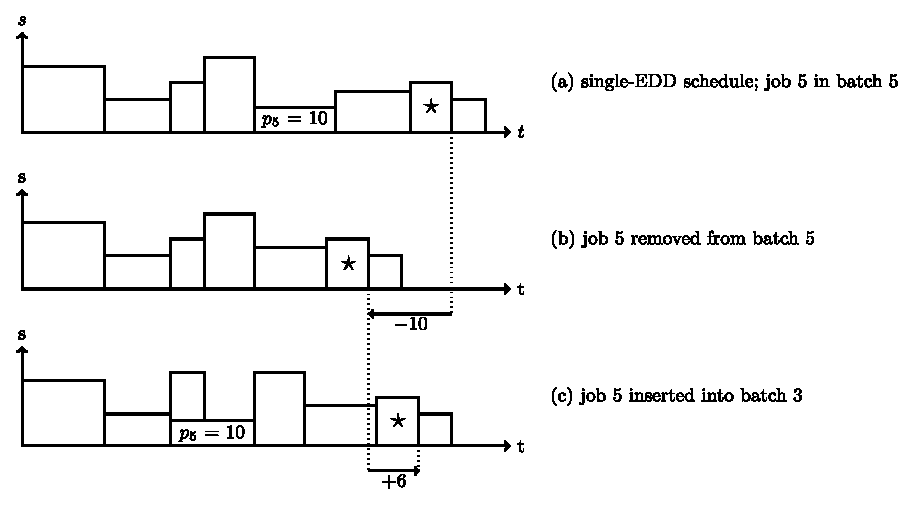
\includegraphics[width=\textwidth]{movebasedmip.pdf}
\caption{Moving a job in a single-EDD schedule. Job 5 (marked
``$p_5 = 10$'') is moved from its single-EDD batch 5 into the earlier batch 3.
This changes the lateness of job 7 (marked $\star$) from $L_\mathrm{7,single}$
to $L_\mathrm{7,single} - 10 + 6 = L_\mathrm{7,single} - 4$.}
  \label{fig:movebasedmip}
\end{figure}

In any batch, only the host job's lateness is relevant to $\Lmax$.
In other words, the lateness of batch $B_k$ equals the lateness of
job $j=k$, unless the job was moved into an earlier batch (in which
case $P_k = 0$ due to Proposition \ref{prop:nohostless} and $L_k = L_{k-1}$). Therefore, we can understand
the lateness of batch $B_k$ as its lateness in the single-EDD schedule, written as
$L_{k,\mathrm{single}}$, modified by the summed effect that all moves of
other jobs into and out of batches $h \leq k$ have on the completion time
of $B_k$:
\begin{alignat}{2}
  \label{c:lmaxc} & L_k = L_{k,\mathrm{single}} + \sum_{h\leq k} \underbrace{P'_h - p_h(2 -
x_{hh})}_{T_h} \quad && \forall k \in \mathcal{B}^\star\\
  \label{c:pkpj} & P'_k \geq p_j x_{jk} \quad && \forall \{j \in \mathcal{J}, k \in \mathcal{B} | j \geq k\} \\
  \label{c:pkmin} & P'_k \geq p_j \quad && \forall \{j \in \mathcal{J}, k \in \mathcal{B} | j = k\}
\end{alignat}
where $P'_k = \max(P_k, p_k) \forall k \in \mathcal{B}$ as defined in
constraints \eqref{c:pkpj} and \eqref{c:pkmin}.

\begin{proposition}
  Constraints \eqref{c:lmaxc}--\eqref{c:pkmin} are sufficient to define $\Lmax$.
\end{proposition}
\begin{proof}
  For every batch $B_k \in \mathcal{B}^\star$, consider the possible scenarios for all batches
$B_h, h \leq k$:
\begin{itemize}
  \item{Batch $B_h$ holds its host job. Then $x_{hh}=1$ and the summand $T_h$ evaluates
      to $P'_h - p_h$. If $B_h$ has guest jobs, then $P'_h - p_h > 0$ if any of
      them are longer than the host job; if all guests are shorter, $P'_h=p_h$
    and $T_h = 0$.}
  \item{Batch $B_h$ is hostless and thus empty. We require $T_h = -p_h$ in
      accordance with Figure \ref{fig:movebasedmip}(b). To achieve this, we
      state in constraints \eqref{c:pkmin} that $P'_h$ never drop below the
      length of its host job, even when $P_h=0$. With this in effect, the
      minimization objective enforces $P'_h = p_h$ and $T_h = P'_h - 2p_h =
    -p_h$.}
\end{itemize}
Effectively thus, we add to $L_k$ the increase in processing time due
to guests, $\max(0, P'_h-p_h)$, for every non-empty batch $B_h$; we
subtract from $L_k$ the host job processing time $p_h$ for every empty
batch $B_h$. This is congruent with Figure \ref{fig:movebasedmip} above.

Note that the $P'_k$ variables used here are not the same as the
physically meaningful $P_k$ due to constraints \eqref{c:pkmin}, which is
why we distinguish them with a prime mark.

Note also that if a batch $B_k \in \mathcal{B}^\star$ is empty, then its
lateness equals that of the previous batch $B_{k-1}$: 
\begin{align*}
L_k =
&\left[L_{{k-1},\mathrm{single}} + P_k - (d_k - d_{k-1})\right] \\&\quad+\left[\sum_{h\leq k-1}
P'_h-p_h(2-x_{hh}) \right] + P'_k - p_k(2-x_{kk}) = L_{k-1}
\end{align*}
as $d_k = d_{k-1}$
and $x_{kk}$ if $B_k$ is empty.

\textbf{$\uparrow\quad$ CB: Your concern about empty batches in
$\mathcal{B}^\star$ makes sense from the old model's perspective. But here every
batch's lateness is defined independently of the previous batch's. I can write
out the math if you think that helps? (I'm worried we don't have the room for it) }


The net sum of these additions and subtractions to and from
$L_{k,\mathrm{single}}$ adjusts the lateness of batch $k$ to its correct number
given the values of $x_{jk}$.
\end{proof}
\pagebreak
We first express the lateness of the first batch as its single-EDD lateness,
plus $\max(P_1 - p_1, 0)$ since guest jobs may cause $P_1 > p_1$:
\begin{equation}
  \label{eq:ind1}
  L_1 = L_{1,\mathrm{single}} + \underbrace{P'_1 -
  p_1(2-x_{11})}_{=\max(P_1-p_1,0)}.
\end{equation}
We then consider the lateness of any batch, $L_k$, which can be written as
\begin{equation}
  \label{eq:ind2}
  L_k = L_{k-1} + \underbrace{P_k}_{C_k-C_{k-1}} - \underbrace{(d_k -
  d_{k-1})}_{D_k-D_{k-1}}.
\end{equation}
Note that we can use the respective host jobs' due dates as the batch due dates
due to Proposition \ref{prop:nohostless}.
We first expand the $L_{k-1}$ term into
\begin{equation}
  \label{eq:ind3}
  L_{k-1} = L_{k-1,\mathrm{single}} + \sum_{h\leq k-1} P'_h - p_h(2-x_{hh}),
\end{equation}
which we know to be true for the case of $k-1 = 1$. We then argue that
\begin{equation}
  \label{eq:ind4}
  P_k - (d_k - d_{k-1}) = L_{k,\mathrm{single}} - L_{k-1,\mathrm{single}} +
\begin{cases}\max(P_k-p_k,0)&x_{kk}=1\\-p_k&x_{kk}=0\end{cases}.
\end{equation}
Note that after substituting \eqref{eq:ind3} and \eqref{eq:ind4} into equation
\eqref{eq:ind2}, the $L_{k-1,\mathrm{single}}$ terms cancel. Finally, the
conditional expression is equivalent to $P'_k - p_k(2-x_{kk})$, and thus
\begin{equation}
  L_k = L_{k,\mathrm{single}} + \left[\sum_{h\leq k-1} P'_h -
  p_h(2-x_{hh})\right] + P'_k - p_k(2-x{kk}),
\end{equation}
which is simply
\begin{equation}
  L_k = L_{k,\mathrm{single}} + \sum_{h\leq k} P'_h - p_h(2 -
x_{hh}).
\end{equation}
\pagebreak
\subsection{Additional lazy constraints}
Additionally, \textit{lazy constraints} \cite{cplexmanual} are used in the model. Lazy
constraints can be generated in the thousands prior to solving, but are
not immediately used in the model. Instead, they are checked
whenever an integral solution is found, and only those that are violated
are added to the LP model. In practice, only few of the lazy constraints
are used in the solution process. Nevertheless, they can noticeably
improve solving time in some cases.

\subsubsection{Symmetry-breaking rule}
This rule creates an explicit, arbitrary preference for certain solutions.
Consider two schedules $S_1$ and
$S_2$. Both schedules contain batches $B_h$ and $B_k$, both of which
are holding their respective host jobs only. Two jobs $j$ and $i$ are now
assigned as the only guests to the two batches; furthermore $\max(p_i, p_j) \leq
\min(p_h, p_k)$, $\max(s_h, s_k) + \max(s_j, s_i) \leq b$ and
$\min(d_j, d_i) \geq \max(d_h, d_k)$. If $j \rightarrow
B_h$ and $i \rightarrow B_k$ in schedule $S_1$ and vice versa in
$S_2$, then the constraint renders $S_2$ infeasible.

\begin{alignat}{2}
  & \begin{gathered} 2 (  4 - x_{hh} - x_{kk} - x_{jh} - x_{jk} -
x_{ih} - x_{ik}\hfill \\+ \sum_{\substack{{g}\\{g \neq j}\\{g \neq
i}}} (x_{gh} + x_{gk}) ) \geq x_{jk} + x_{ih} \end{gathered}
\quad && \begin{gathered} \forall\{ j, i \in \mathcal{J}, \\ h, k \in K \\|\; h < k <
j < i \land \\ [p_i \leq k_h \land b - s_h \geq s_i\\ \forall i \in
\{j,i\}, \\ \forall h
\in \{h,k\}] \} \end{gathered}
\end{alignat}

The left-hand side of the equation evaluates to zero exactly when the above
conditions are met, which in turn disallows the assignment given on the right.
For all other job/batch pairings, the left side evaluates to at least two, which
places no constraint on the right hand side at all.

This kind of symmetry-breaking rule can theoretically be extended to situations with
$m > 2$ batches, with the number of constraints growing combinatorially with $m$. Since it takes
a constant but appreciable time to generate these constraints prior to solving,
we have in our trials kept to the simplest variant shown here, and limited their
use to problem instances with $n \geq 50$ jobs.

\subsubsection{Dominance rule on required assignments}
A schedule is not uniquely optimal if a job $j$ is left in its single-EDD batch
although there is capacity for it in an earlier batch. This constraint can
be expressed logically as: if a job $j$ can be safely assigned to $B_k$ without
violating the capacity constraint, then $j$ must be moved somewhere, or
$B_k$ must be empty (or both). 

The left side of the above \textit{if-then} statement is written as $(1.0 + b -
s_j - \sum_{\substack{{i = k}\\{i \neq j}}}^{n_j} s_i x_{ik}) / b$, which
evaluates to 1.0 or greater iff $s_k$ plus the sizes of guest jobs in $k$ sum to
less than $b - s_j$. The constraint is written as follows:
\begin{alignat}{2}
&2 - x_{jj} - x_{kk} \geq \left(1.0 + b - s_j -
\sum_{\substack{{i = k}\\{i \neq j}}}^{n_j} s_i
x_{ik}\right) / b \quad && \begin{gathered} \forall \{k \in \mathcal{B}, j \in \mathcal{J} \\| j > k 
\land p_k \geq p_j \\ \land s_k + s_j \leq b\}\end{gathered}
\end{alignat}\\

As with the rule above, we have found that only more difficult problems with $n
\geq 50$ benefit from these constraints.

\section{A New MIP Model}
\label{sec:newMIPmodel}

The full novel MIP model we are proposing is defined in Model \ref{mod:movebackmip}.

\begin{model}
\begin{alignat}{2}
\mathrm{Min.}\quad & \Lmax && \\
\mathrm{s.t.}\quad & \label{mbm:eq7}\sum_{k} x_{jk} = 1 \quad && \forall j \in \mathcal{J} \\
& \label{mbm:eq6}\sum_{j} s_j x_{jk} \leq b \quad && \forall k \in \mathcal{B} \\
&\label{mbm:eq3} P'_k \geq p_j x_{jk} \quad && \forall \{j \in \mathcal{J}, k \in \mathcal{B} | j \geq k\} \\
&\label{mbm:eq10} P'_k \geq p_j \quad && \forall \{j \in \mathcal{J}, k \in \mathcal{B} | j = k\} \\
&\label{mbm:eq5} x_{kk} \geq x_{jk} \quad && \forall \{j \in \mathcal{J}, k \in \mathcal{B} | j > k\} \\
&\label{mbm:eq4} \Lmax \geq L_{k,\mathrm{single}} + \sum_{h\leq k} P'_h - p_h(2 -
x_{hh}) \quad && \forall k \in \mathcal{B}^\star \\
  \label{mbm:eq1} & x_{jk} = 0 \quad && \forall \{j \in \mathcal{J}, k \in \mathcal{B} | j < k\}
  \\[2ex]
  (*)\quad \label{mbm:eq8} & \begin{gathered} 2 (  4 - x_{k_1,k_1} - x_{k_2,k_2} - x_{j_1,k_1} - x_{j_1,k_2} -
x_{j_2,k_1} - x_{j_2,k_2}\hfill \\+ \sum_{\substack{{j}\\{j \neq j_1}\\{j \neq
j_2}}} (x_{j,k_1} + x_{j,k_2}) ) \geq x_{j_1,k_2} + x_{j_2,k_1} \end{gathered}
\quad && \begin{gathered} \forall\{ j_1, j_2 \in \mathcal{J}, \\ k_1, k_2 \in K \\|\; k_1 < k_2 <
j_1 < j_2 \land \\ [p_i \leq k_h \land b - s_h \geq s_i\\ \forall i \in
\{j_1,j_2\}, \\ \forall h
\in \{k_1,k_2\}] \} \end{gathered}
 \\[2ex]
(*)\quad &  \label{mbm:eq11}2 - x_{jj} - x_{kk} \geq \left(1.0 + b - s_j -
\sum_{\substack{{i = k}\\{i \neq j}}}^{n_j} s_i
x_{ik}\right) / b \quad && \begin{gathered} \forall \{k \in \mathcal{B}, j \in \mathcal{J} \\| j > k 
\land p_k \geq p_j \\ \land s_k + s_j \leq b\}\end{gathered}
\end{alignat}
\caption{Move-based MIP model. Constraints marked $(*)$ are lazy constraints.}
\label{mod:movebackmip}
\end{model}

Constraints \eqref{mbm:eq7} and \eqref{mbm:eq6} are uniqueness and
capacity constraints: batches have to remain within capacity $b$, and every
job can only occupy one batch.

Constraints \eqref{mbm:eq3} and \eqref{mbm:eq10} define the value of
$P_k$ for every batch $k$ as the longest $p$ of all jobs in $k$, but
at least $p_k$. This is required in \eqref{mbm:eq4}, which follows the
explanation above.

Constraints \eqref{mbm:eq5} ensure that no job is moved into a host-less batch,
i.e. in order to move job $j$ into batch $k$ ($x_{jk} = 1$), job $k$ must still
be in batch $k$ ($x_{kk} = 1$).

Constraints \eqref{mbm:eq1} implement the requirement that jobs are only moved
into earlier batches.

Constraints \eqref{mbm:eq8} and \eqref{mbm:eq11} implement the additional lazy
constraints described above.

\section{Empirical comparison}
\label{sec:exp}

We empirically compared the performance of the CP model by Malapert et al. and
Model \ref{mod:movebackmip}. Both models were run on 120
benchmark instances provided by Malapert et al. (i.e. 40 instances of each $n_j = \{20,
50, 75\}$). The benchmarks are generated as specified in \cite{Daste1}, with a
capacity of $b = 10$ and values for $p_j$, $s_j$ and $d_j$ distributed as follows:
\begin{align}
p_j &= U[1, 99] \\
s_j &= U[1, 10] \\
d_j &= U[0, 0.1] \cdot \tilde{C}_\text{max} + U[1, 3] \cdot p_j
\end{align}
where $U[a, b]$ is a uniform distribution between $a$ and $b$, and
$\tilde{C}_\text{max} = \frac{1}{bn} \cdot \\ \left( \sum_{j=1}^{n_j} s_j \cdot \sum_{j=1}^{n_j}
p_j \right)$ is an approximation of the time required to process
all jobs.

The MIP benchmarks were run using \textsc{cplex} 12.5 \cite{cplex} on an Intel
i7 Q740 CPU (1.73 GHz) and 8 GB RAM in single-thread mode, with \textsc{cplex}
parameters \texttt{Probe = Aggressive} and \texttt{MIPEmphasis = Optimality}
(the latter for $n=20$ only). The CP was implemented using the Choco solver library \cite{choco} and run on the same
machine using the same problem instances.\footnote{The authors would like to extend a warm
  thank-you to Arnaud Malapert for both providing his code and helping us run
it.}
Solving was aborted after a time of 3600 seconds (1 hour).

The reference MIP model solves less than a third of all instances to optimality
within the time limit. The branch-and-price model proposed by Daste \cite{Daste1} also
performs considerably worse than CP \cite{Malapert}. Neither of the two is
included in these results.

\subsection{Results}
The overview in Table \ref{table:results} below shows aggregated results that
demonstrate the performance and robustness of our new model.

\small
\begin{table}
\noindent\begin{tabu} to \linewidth {l l X[r] X[r] X[r] X[r] X[r]}
  \toprule
  \multirow{2}{*}{$n_j$}& \multirow{2}{*}{optimal soln. found by} &
  \multirow{2}{*}{instances} &
\multicolumn{2}{r}{solving time [s]} & \multicolumn{2}{r}{
absolute gap} \\
   & & & CP & MIP & CP & MIP \\
  \toprule
  20\;\; & both models & 40/40 & 0.42 & 0.04 & 0 & 0 \\
  \midrule
  50 & both models & 40/40 & 5.67 & 4.16 & 0 & 0 \\
  \midrule
  \multirow{4}{*}{75} & both models & 22/40 & 49.30 & 52.88
  & 0 & 0 \\
  & CP model only & 0/40 & --- & --- & --- & --- \\
  & MIP model only & 13/40 & $>3600$ & 139.86 & 323.46 & 0
  \\
  & neither model & 5/40 & $>3600$ & $>3600$ & 310.40 & 25.00 \\
  \bottomrule
\end{tabu}
\vspace{0.3em}
\caption{Summary of empirical results. Values are geometric means for solving
  time and arithmetic means for absolute gaps. Note that no relative gaps are given
  because negative lower bounds result in misleading percentages; see Figure
\ref{fig:gapcomp} for a more detailed gap comparison.}
\label{table:results}
\end{table}
\normalsize
As shown in Figure \ref{fig:scattercomp}, our MIP model performed better overall on
instances with $n_j = 20$ and $n_j = 75$, while MIP and CP perform similarly
well on intermediate problems ($n_j = 50$).

Wherever an optimal solution was not found within the 1-hour time limit,
the improved MIP model achieved a significantly better solution quality: 
out of the 40 instances with $n_j = 75$, 22 were solved to optimality by both CP
and MIP, 13 were solved to optimality by the MIP only, and 5
were solved by neither model within an hour. 

\begin{figure}[h]
\centering
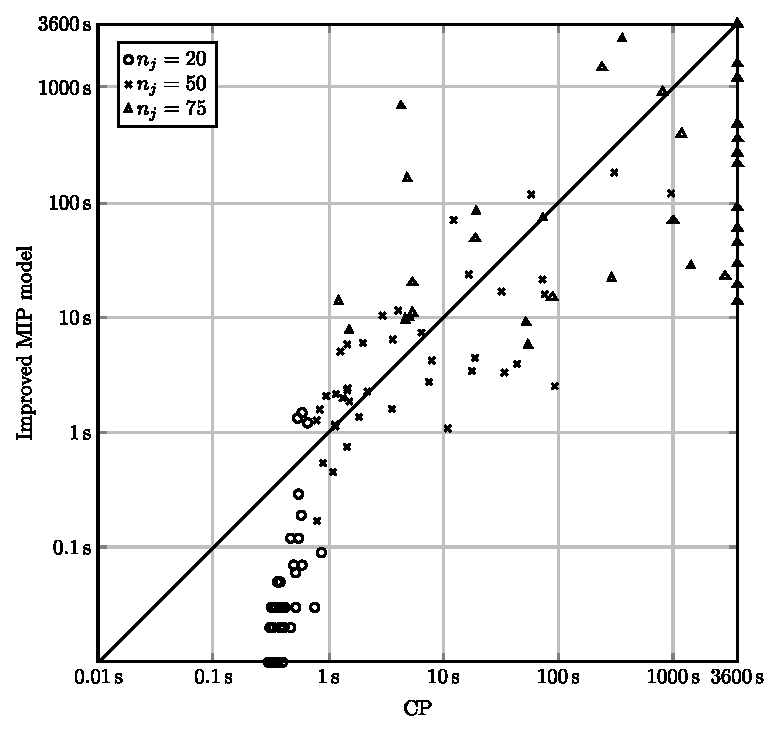
\includegraphics[height=0.55\textheight]{scattercomp.pdf}
\caption{Performance comparison over 120 instances, each represented by one data
point. Horizontal/vertical coordinates correspond to solving time by CP model
and improved MIP model, respectively. Note that 16 instances were not solved to
optimality within an hour by either the CP model or both models.}
\label{fig:scattercomp}
\end{figure}

\begin{figure}[h]
\centering
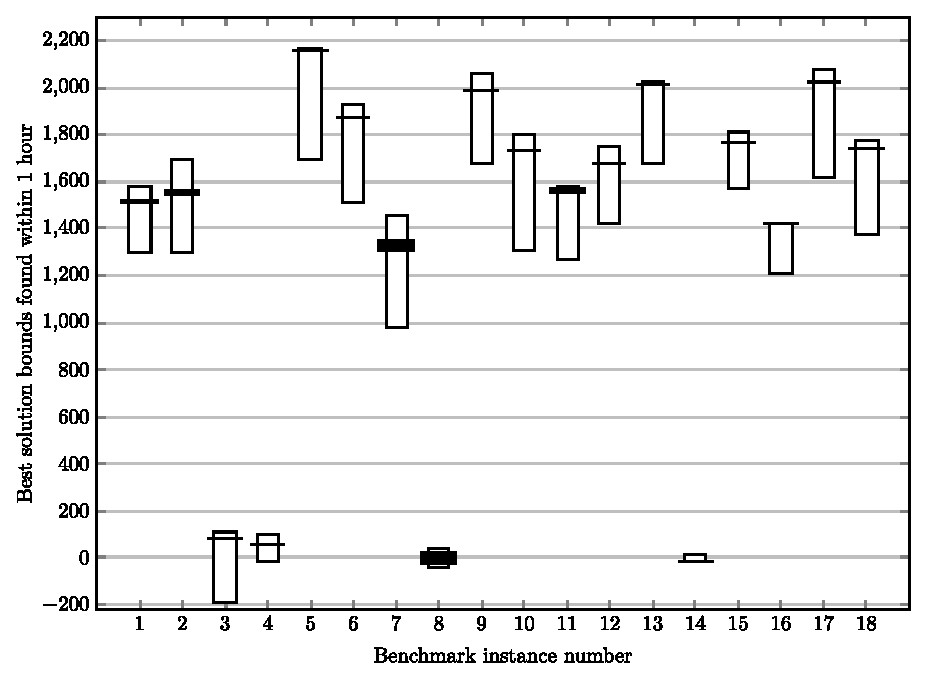
\includegraphics[height=0.45\textheight]{gapcomp.pdf}
\caption{Comparison of solution quality for the 18 instances that were not
solved to optimality within an hour by either the CP model or both models. White bars represent
the LB-UB gap achieved by the CP model, black bars the LB-UB gap achieved by the
improved MIP model (straight line if solved to optimality).}
\label{fig:gapcomp}
\end{figure}

\section{Discussion}
\label{sec:discussion}
Our results show that the improved MIP model is an improvement over previous
approaches, demonstrating that at least in this case, the performance
of custom implementations can indeed be matched and exceeded by
a comparatively simple mathematical formulation.

A comparison of solution quality where no optimal schedule was
found confirms the robustness of the improved MIP model: as Figure
\ref{fig:gapcomp} illustrates, the gap (UB($\Lmax)-$LB($\Lmax$)) is
consistently larger in the CP model. This means that even with very difficult
problems, our model will often give near-optimal solutions more quickly
than Malapert et al.'s CP model.

Mathematical models also have the general benefit of being more readily
understandable, straightforward to implement and reasonably easy to
adapt to new, similar problems.

\subsection{Correlation between problem configuration and solving time}
\label{sec:correlation}
The mean number of jobs per batch ($n_j/n_k$) in the optimal solution
strongly correlates with the time needed to solve to optimality. This
is unsurprising given that a problem with a great number of large jobs
(i.e. large $s_j$) will be of relatively low difficulty in terms of bin
packing. 

An excellent predictor of solving time therefore appears to be what Baptiste \& LePape
\cite{baptistelepape} call the \textit{disjunction ratio}: the ratio between the
number of job pairs which cannot run in parallel (as $s_{j_1} + s_{j_2} > b$) and
the total number of job pairs $n_j^2$. For a sample of 40 random instances of
$n_j=30$, we found a correlation between $n_j/n_k$ and solution time of $r =
0.72$ and a correlation between disjunction ratio and solution time of $r =
-0.64$.

As a corollary, the solving time is greatly dependent on the
capacity of the machine. Larger capacities, relative to the average job size
$\bar{s}_j$, will correlate with longer solving times as the disjunction ratio decreases.

\subsection{Generalizing the search technique used in the improved MIP model}

The effects of binary decision variables on the objective function can often be
considered discretely, which allows us to reason about them algorithmically
even though they constitute an entirely declarative model.
Indeed, the concept of \textit{moves} typically appears
in local search techniques, such as the \textit{Large Neighbourhood
Search} \cite{shaw} where moves correspond to the removal and
re-insertion of jobs from and into the schedule, similarly to what
we propose in Section \ref{sec:moves} above. Analogous to the notion
of ``neighbourhood'' is the set of schedules than can be reached via
feasible moves, starting from any other schedule. We can then easily
represent the objective function as a sum of changes from
some canonical solution. Such models, while non-standard, may provide
substantial insight into problem structure that can be exploited in a
MIP (or CP) formulation.

\section{Conclusion} 
\label{sec:conclusion}

\textbf{CB: Needs rewriting later.}

By examining the batch scheduling problem carefully, we were able to identify
redundancies in the original model. We proposed a new model and showed that its
performance is comparable to, or better than that of the state-of-the-art
constraint programming implementation.

\bibliography{bibliography}{}
\bibliographystyle{splncs}


\end{document}
